% Options for packages loaded elsewhere
\PassOptionsToPackage{unicode}{hyperref}
\PassOptionsToPackage{hyphens}{url}
%
\documentclass[
  english,
  man]{apa6}
\usepackage{lmodern}
\usepackage{amssymb,amsmath}
\usepackage{ifxetex,ifluatex}
\ifnum 0\ifxetex 1\fi\ifluatex 1\fi=0 % if pdftex
  \usepackage[T1]{fontenc}
  \usepackage[utf8]{inputenc}
  \usepackage{textcomp} % provide euro and other symbols
\else % if luatex or xetex
  \usepackage{unicode-math}
  \defaultfontfeatures{Scale=MatchLowercase}
  \defaultfontfeatures[\rmfamily]{Ligatures=TeX,Scale=1}
\fi
% Use upquote if available, for straight quotes in verbatim environments
\IfFileExists{upquote.sty}{\usepackage{upquote}}{}
\IfFileExists{microtype.sty}{% use microtype if available
  \usepackage[]{microtype}
  \UseMicrotypeSet[protrusion]{basicmath} % disable protrusion for tt fonts
}{}
\makeatletter
\@ifundefined{KOMAClassName}{% if non-KOMA class
  \IfFileExists{parskip.sty}{%
    \usepackage{parskip}
  }{% else
    \setlength{\parindent}{0pt}
    \setlength{\parskip}{6pt plus 2pt minus 1pt}}
}{% if KOMA class
  \KOMAoptions{parskip=half}}
\makeatother
\usepackage{xcolor}
\IfFileExists{xurl.sty}{\usepackage{xurl}}{} % add URL line breaks if available
\IfFileExists{bookmark.sty}{\usepackage{bookmark}}{\usepackage{hyperref}}
\hypersetup{
  pdftitle={Reproducing the analysis of Pfattheicher et al., (2020)},
  pdfauthor={Kristina Arevalo1},
  pdflang={en-EN},
  pdfkeywords={COVID-19, pandemic, face masks, empathy},
  hidelinks,
  pdfcreator={LaTeX via pandoc}}
\urlstyle{same} % disable monospaced font for URLs
\usepackage{graphicx,grffile}
\makeatletter
\def\maxwidth{\ifdim\Gin@nat@width>\linewidth\linewidth\else\Gin@nat@width\fi}
\def\maxheight{\ifdim\Gin@nat@height>\textheight\textheight\else\Gin@nat@height\fi}
\makeatother
% Scale images if necessary, so that they will not overflow the page
% margins by default, and it is still possible to overwrite the defaults
% using explicit options in \includegraphics[width, height, ...]{}
\setkeys{Gin}{width=\maxwidth,height=\maxheight,keepaspectratio}
% Set default figure placement to htbp
\makeatletter
\def\fps@figure{htbp}
\makeatother
\setlength{\emergencystretch}{3em} % prevent overfull lines
\providecommand{\tightlist}{%
  \setlength{\itemsep}{0pt}\setlength{\parskip}{0pt}}
\setcounter{secnumdepth}{-\maxdimen} % remove section numbering
% Make \paragraph and \subparagraph free-standing
\ifx\paragraph\undefined\else
  \let\oldparagraph\paragraph
  \renewcommand{\paragraph}[1]{\oldparagraph{#1}\mbox{}}
\fi
\ifx\subparagraph\undefined\else
  \let\oldsubparagraph\subparagraph
  \renewcommand{\subparagraph}[1]{\oldsubparagraph{#1}\mbox{}}
\fi
% Manuscript styling
\usepackage{upgreek}
\captionsetup{font=singlespacing,justification=justified}

% Table formatting
\usepackage{longtable}
\usepackage{lscape}
% \usepackage[counterclockwise]{rotating}   % Landscape page setup for large tables
\usepackage{multirow}		% Table styling
\usepackage{tabularx}		% Control Column width
\usepackage[flushleft]{threeparttable}	% Allows for three part tables with a specified notes section
\usepackage{threeparttablex}            % Lets threeparttable work with longtable

% Create new environments so endfloat can handle them
% \newenvironment{ltable}
%   {\begin{landscape}\begin{center}\begin{threeparttable}}
%   {\end{threeparttable}\end{center}\end{landscape}}
\newenvironment{lltable}{\begin{landscape}\begin{center}\begin{ThreePartTable}}{\end{ThreePartTable}\end{center}\end{landscape}}

% Enables adjusting longtable caption width to table width
% Solution found at http://golatex.de/longtable-mit-caption-so-breit-wie-die-tabelle-t15767.html
\makeatletter
\newcommand\LastLTentrywidth{1em}
\newlength\longtablewidth
\setlength{\longtablewidth}{1in}
\newcommand{\getlongtablewidth}{\begingroup \ifcsname LT@\roman{LT@tables}\endcsname \global\longtablewidth=0pt \renewcommand{\LT@entry}[2]{\global\advance\longtablewidth by ##2\relax\gdef\LastLTentrywidth{##2}}\@nameuse{LT@\roman{LT@tables}} \fi \endgroup}

% \setlength{\parindent}{0.5in}
% \setlength{\parskip}{0pt plus 0pt minus 0pt}

% \usepackage{etoolbox}
\makeatletter
\patchcmd{\HyOrg@maketitle}
  {\section{\normalfont\normalsize\abstractname}}
  {\section*{\normalfont\normalsize\abstractname}}
  {}{\typeout{Failed to patch abstract.}}
\patchcmd{\HyOrg@maketitle}
  {\section{\protect\normalfont{\@title}}}
  {\section*{\protect\normalfont{\@title}}}
  {}{\typeout{Failed to patch title.}}
\makeatother
\shorttitle{Reproducing the analysis of Pfattheicher et al., (2020)}
\keywords{COVID-19, pandemic, face masks, empathy}
\DeclareDelayedFloatFlavor{ThreePartTable}{table}
\DeclareDelayedFloatFlavor{lltable}{table}
\DeclareDelayedFloatFlavor*{longtable}{table}
\makeatletter
\renewcommand{\efloat@iwrite}[1]{\immediate\expandafter\protected@write\csname efloat@post#1\endcsname{}}
\makeatother
\usepackage{lineno}

\linenumbers
\usepackage{csquotes}
\ifxetex
  % Load polyglossia as late as possible: uses bidi with RTL langages (e.g. Hebrew, Arabic)
  \usepackage{polyglossia}
  \setmainlanguage[]{english}
\else
  \usepackage[shorthands=off,main=english]{babel}
\fi

\title{Reproducing the analysis of Pfattheicher et al., (2020)}
\author{Kristina Arevalo\textsuperscript{1}}
\date{}


\authornote{

Kristina Arevalo, Department of Psychology, Brooklyn College of the City University of New York.

The authors made the following contributions. Kristina Arevalo: .

Correspondence concerning this article should be addressed to Kristina Arevalo, 1126 E 72nd St. E-mail: \href{mailto:krisarevalo29@gmail.com}{\nolinkurl{krisarevalo29@gmail.com}}

}

\affiliation{\vspace{0.5cm}\textsuperscript{1} Brooklyn College of the City University of New York}

\abstract{
A reproduction of the analysis for Study 4 from Pfattheicher et al., (2020).
}



\begin{document}
\maketitle

Pfattheicher, Nockur, Böhm, Sassenrath, and Petersen (2020) wanted to know if physical distancing and the wearing of face masks are due to empathy for people most vulnerable to the virus. In study 4, state empathy was assessed after each participant was assigned to either an empathy condition, an information-only condition, or a control condition. This was to prove empirically that higher levels of state empathy are directly related to the motivation to adhere to COVID-19 measures.

\newpage

\hypertarget{methods}{%
\section{Methods}\label{methods}}

\hypertarget{participants}{%
\subsection{Participants}\label{participants}}

This study had a total of 1,526 participants; 47.2\% female; age: M = 34.71 years, SD = 12.09) and was run in Germany between June 23 and June 26, 2020. Each participant was randomly assigned to one of three conditions: the information-only condition (n = 492), the empathy condition (n = 500), or the control condition (n = 534).

\hypertarget{procedure}{%
\subsection{Procedure}\label{procedure}}

Participants in the information-only condition read an informative text from the Robert Koch Institute detailing facts about the coronavirus, how it is transmitted, and that face masks can prevent the spread of the disease. Participants in the empathy condition read a text of approximately similar length, in which a woman with a rare immune disease reported having had a coronavirus infection, detailed how seriously affected she was, and stated that she did not like it when people met others without wearing a face mask. In the control condition, no text and information were given, resembling a situation of no intervention. After the condition manipulations, participants responded to three items assessing state empathy. The central dependent variable was motivation to wear a face mask, which was measured with one item: \enquote{During the coming days, I will wear a face mask as often as possible when I meet other people.}

\newpage

\hypertarget{results}{%
\section{Results}\label{results}}

\hypertarget{read-and-clean-the-data}{%
\subsection{Read and Clean the Data}\label{read-and-clean-the-data}}

\begin{verbatim}
## NULL
\end{verbatim}

\hypertarget{independent-sample-t-tests}{%
\subsection{Independent Sample t-tests}\label{independent-sample-t-tests}}

\hypertarget{one-way-anova}{%
\subsection{One-way ANOVA}\label{one-way-anova}}

\hypertarget{figure-3-replication}{%
\subsection{Figure 3 Replication}\label{figure-3-replication}}

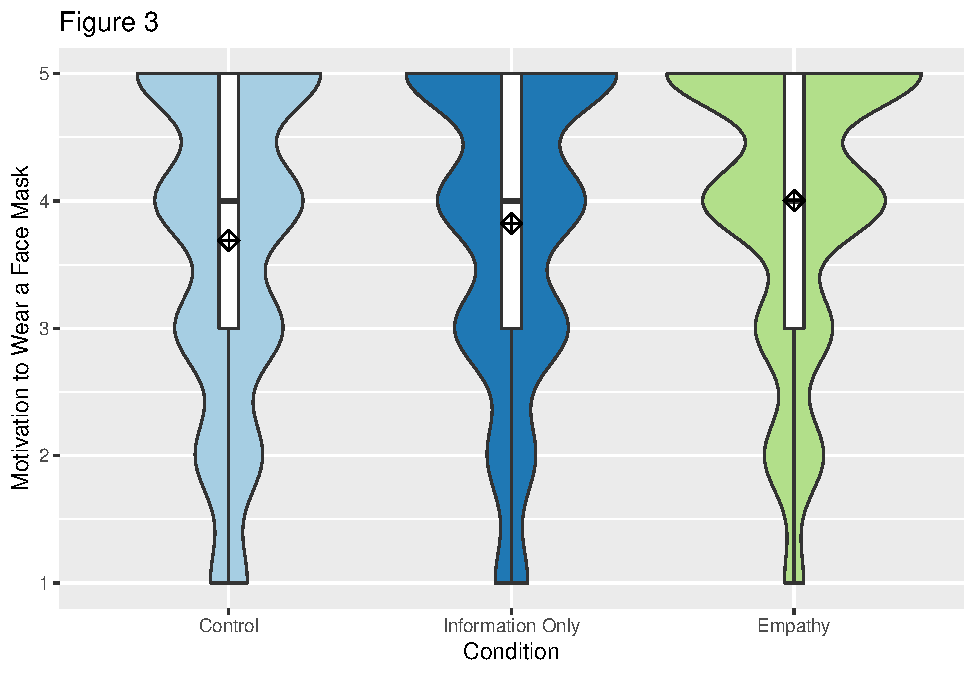
\includegraphics{APA_Report_files/figure-latex/unnamed-chunk-6-1.pdf}

\hypertarget{papaja-reporting}{%
\subsection{Papaja Reporting}\label{papaja-reporting}}

I found that participants in the empathy condition reported significantly higher state-empathy levels compared with the information-only condition,\(\Delta M = 1.89\), 95\% CI \([1.77\), \(2.00]\), \(t(990) = 31.22\), \(p < .001\), and compared with the control condition \(\Delta M = 1.93\), 95\% CI \([1.82\), \(2.05]\), \(t(1,032) = 32.41\), \(p < .001\). The information-only and the control conditions did not differ significantly, \(\Delta M = -0.05\), 95\% CI \([-0.17\), \(0.08]\), \(t(1,024) = -0.76\), \(p = .448\). A one-way ANOVA showed that the motivation to wear a mask also differed between conditions, \(F(2, 1,523) = 8.97\), \(\mathit{MSE} = 1.41\), \(p < .001\), \(\hat{\eta}^2_G = .012\)

\hypertarget{discussion}{%
\section{Discussion}\label{discussion}}

The re-analysis successfully reproduced the analysis reported by Pfattheicher et al., (2020). In study 4 of their experiment, they conducted several t-tests and a one-way ANOVA which were all successfuly reproduced. In the following section, I show an example of completing a simulation based power analysis for this design.

\hypertarget{simulation-based-power-analysis}{%
\subsection{Simulation-based power analysis}\label{simulation-based-power-analysis}}

The design was a between subject design with 1,526 subjects. This power curve applies for independent-sample t-tests with n=508. Because the groups were unbalanced, a harmonic mean of 508 was computed. Pfattheicher et al. (2020) reported \enquote{With this sample size, we are able to detect effects (fs) greater than .09 with high statistical power (power = .90; alpha = .05, two- tailed).} I believe that based on this power analysis, their study was not under powered.

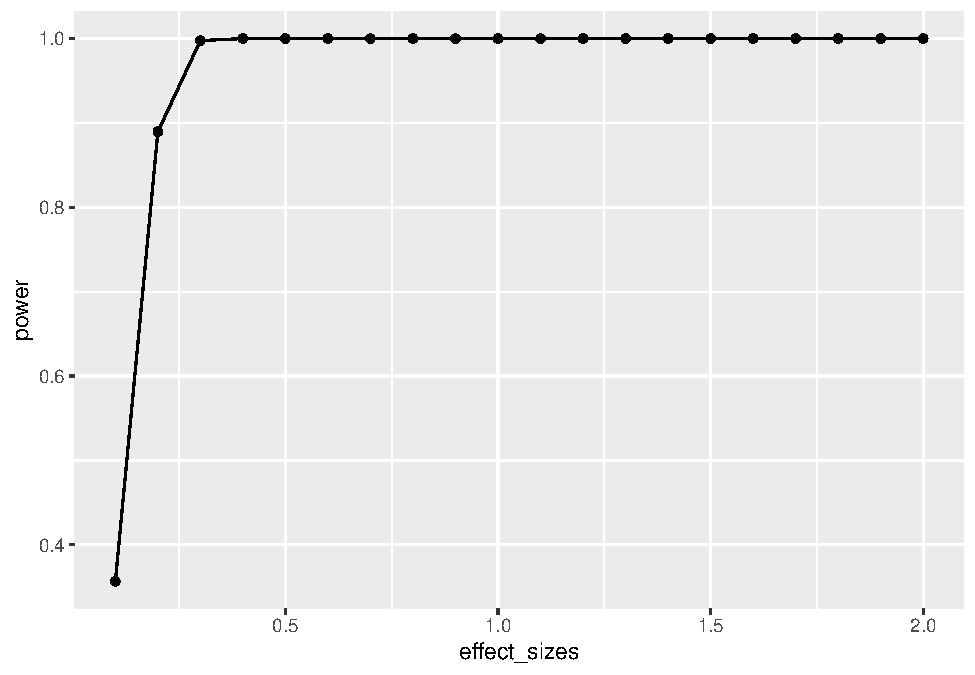
\includegraphics{APA_Report_files/figure-latex/unnamed-chunk-7-1.pdf}

\newpage

\hypertarget{references}{%
\section*{References}\label{references}}
\addcontentsline{toc}{section}{References}

\hypertarget{refs}{}
\leavevmode\hypertarget{ref-pfattheicher_emotional_2020}{}%
Pfattheicher, S., Nockur, L., Böhm, R., Sassenrath, C., \& Petersen, M. B. (2020). The emotional path to action: Empathy promotes physical distancing and wearing of face masks during the COVID-19 pandemic. \emph{Psychological Science}, \emph{31}(11), 1363--1373.


\end{document}
